\section{Introduction}\label{sec:intro}

Spatial and immersive audio techniques have been the beneficiaries of
significant research interest over the past few decades.
Recent explosions in virtual and augmented reality technologies and
\textit{object-based} audio have led to an acceleration in interest in the
creation of virtual sound fields via approaches such as Wave Field Synthesis
(WFS) and Higher Order Ambisonics (HOA)\cite{}.
These techniques call for the deployment of large numbers of loudspeakers, and
centralised, \textit{in situ} installations of dedicated hardware and software.
The costs associated with such installations have seen them largely restricted
to the preserve of concert venues, cinemas, and institutions with the means to
purchase and operate monolithic systems of this sort.

Advancements in embedded computing mean that there now exist an assortment of
small, low-cost devices with support for audio digital signal processing (DSP).
These devices are open source, relatively easy to program, and may provide
support for communication over ubiquitous computer networking equipment and
protocols.
A network of such devices could be used to \textit{distribute} the problem of
audio spatialisation, potentially lowering the barrier to entry to what is
otherwise a comparatively exclusive branch of audio research.

The work that this article describes is an exploration of the possibility of
achieving such an outcome.
As such, it is concerned primarily with the transmission of digital audio
signals throughout a computer network.
It is meaningful, then, to reflect on the nature of such signals, a selection
of their properties of greatest pertinence to this work, and the representation
of audio signals within computer systems and networks.

\subsection{Digital Audio Signals}
\label{subsec:digital-audio-signals}

In a digital audio system with sampling rate $F_s$, an audio signal $y$ is
composed of samples $y[n]$, each representing the amplitude of the signal at a
given point in time $t$, where $t = n/F_s$.
For arithmetical convenience, sample amplitudes are typically treated as
floating point numbers, constrained to the interval $y \in [-1, 1]$ (see
\figref{fig:signal-samples}).
It is in this form that audio samples are typically handled during the
processing stage of a DSP algorithm, and the underlying representation
\textemdash{} that required by low level software and hardware systems
\textemdash{} is concealed; matters of numerical resolution and precision are,
by-and-large, abstracted away.

\begin{figure}[ht]
    \centering
    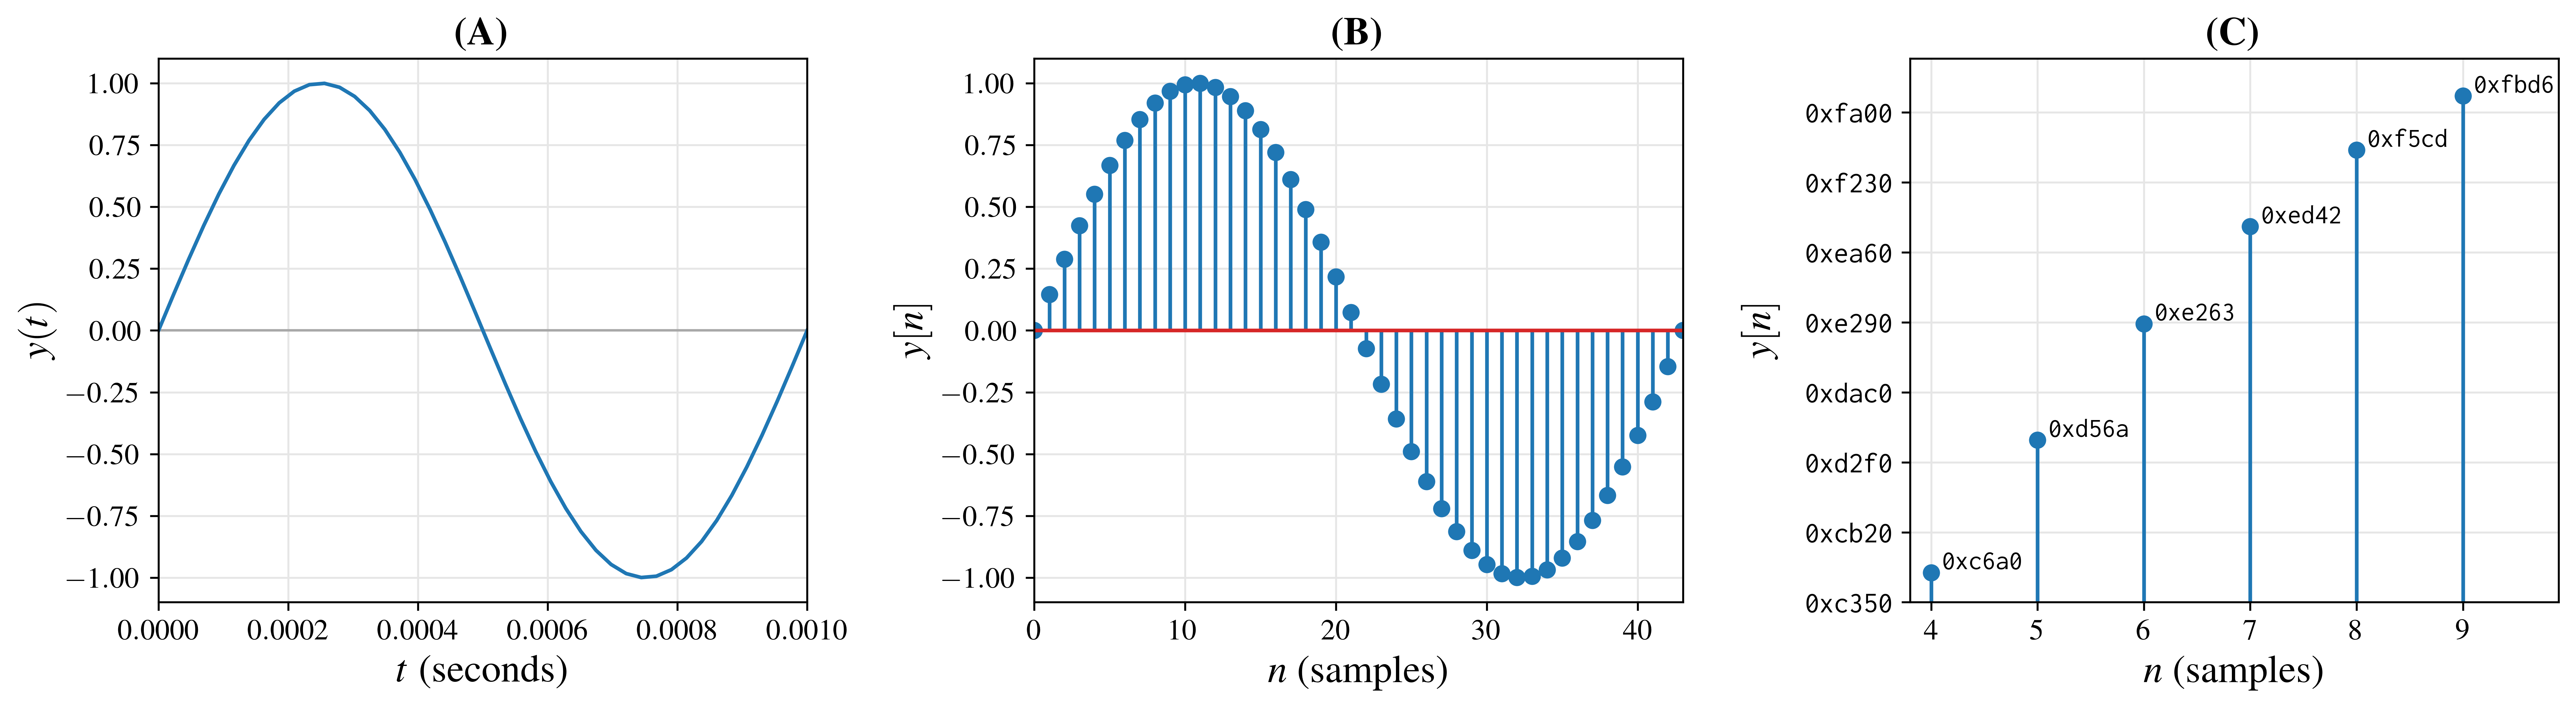
\includegraphics[width=\textwidth]{figures/digital-signal}
    \caption{
        An audio signal (\qty{1}{\kHz} sine wave);
        (a) in continuous time;
        (b) sampled at intervals of $1/Fs$ seconds, with
        $F_s =$~\qty{44.1}{\kHz}.
    }
    \label{fig:signal-samples}
\end{figure}

Samples undergo format conversion at various stages during processing, such as
from an integer pulse code modulation (PCM) filetype to a stream of floating
point audio samples in a digital audio workstation (DAW), or from a floating
point audio stream in an audio device driver to an integer stream to be handled
by a hardware codec.
For the most part, the user, and even the developer of audio software, need not
concern themselves with the rudiments of sample representation and conversion;
as shall be shown, however, under certain circumstances these fundamental
aspects of digital audio systems must be dealt with directly.

\subsection{Numerical Representation}\label{subsec:numerical-representation}

Digital audio samples are ultimately described as binary numbers.
Broadly speaking, the more binary digits (\textit{bits}) available for each
sample, the greater the resolution in terms of distinct amplitudes that can be
represented, with ramifications for dynamic range and signal-to-noise ratio, as
well as for storage and throughput.
Integer sample formats, such as commonly-encountered 16 and 24 bit, offer
comparatively poor resolution at low amplitudes due to the incongruity between
the linear distribution of their values versus the logarithmic nature of sound
intensity.
Floating point formats, by contrast, feature a logarithmic distribution of
available values; the IEEE standard for single-precision (i.e.\ 32 bit) floating
point numbers\cite{} dictates that precision is greatest close to zero,
with around half the available numbers lying in the interval $[-1, 1]$.
